
\begin{exercise}{\emph{(2.6 nel testo)}}
  Considerate il modello in cui $Y_1,\ldots, Y_n$ sono indipendenti e
  identicamente distribuite come una uniforme $Y \sim U(0, \theta)$,
  dove $\theta$ \`e il valore massimo che pu\`o assumere $Y$.
  Determinate per simulazione la distribuzione campionaria di $T = 2Y$
  considerando $\theta = 100, n = 20$. Mostrate con un istogramma che
  la distribuzione dello stimatore \`e approssimabile da una
  normale. Qual \`e la varianza di $T$? Usate questa varianza per
  sovrapporre all'istogramma la curva normale che lo approssima
  (ricordate di disegnare l'istogramma in R con l'opzione freq =
  FALSE).
\end{exercise}
Questo il codice che implementa l'esercizio:
\lstinputlisting{r-sources/exercises/chapter-two/two-six.R}
Vediamo qualche risultato inserendo in R:
\begin{lstlisting}
  > twosix()
  $estimatorVector
    [1]  95.96794 105.40497 110.64482  89.14495 107.99978 116.03221
    94.73158 ...
  
  $empiricalMean
  [1] 100.2173

  $empiricalVar
  [1] 168.8848

  $empiricalVarComputedByHand
  [1] 168.8848

  $sd
  [1] 12.99557
\end{lstlisting}
L'esecuzione della funzione produce la \autoref{fig:two-six}, dove la
curva in blu rappresenta la densit\`a inferita usando gli algoritmi
disponibili in R dello stimatore $2\bar{Y}$, mentre la curva in rosso
rappresenta il modello esatto usando come parametri i valori stimati
dalla media e dalla varianza campionaria (riportate nel precedente
output come \texttt{empiricalMean} e \texttt{empiricalVar}).
\begin{figure}[htb]
\centering
\includegraphics[height=13cm,width=13cm]{r-sources/exercises/chapter-two/two-six.ps}
\caption{Istogramma esercizio 2.6 del testo}
\label{fig:two-six}
\end{figure}

\begin{exercise}{\emph{(2.7 nel testo)}}
  Una azienda chimica ha prodotto un additivo per la benzina che
  dovrebbe migliorare il consumo oltre le 25 miglia per
  gallone. Viene fatto un esperimento con 30 auto uguali su un
  percorso standard e si ottiene un consumo medio di 26.3 mpg con una
  deviazione standard campionaria di 2.4 mpg. Trovare un intervallo di
  confidenza al $95\%$ per il consumo medio supponendo il modello normale.
\end{exercise}
Questo il codice che implementa l'esercizio:
\lstinputlisting{r-sources/exercises/chapter-two/two-seven.R} Nel
campionamento ripetuto l'intervallo di confidenza riportato sotto
conterr\`a il vero valore del parametro (consumo medio) con una
probabilit\`a di copertura del 95\%.
\begin{lstlisting}
  > twoSeven()
  $tOss
  [1] 2.04523
  
  $lower
  [1] 25.40383

  $upper
  [1] 27.19617
\end{lstlisting}

\begin{exercise}{\emph{(2.8 nel testo)}}
  Un misuratore del tasso di alcool nel sangue viene verificato su un
  campione di prova in cui la misura dovrebbe essere 12\%. Trovare una
  stima della media e il suo errore standard. Trovare un intervallo di
  confidenza a livello del 95\% per la media col modello normale. Fare
  un test dell'ipotesi che il misuratore sia correttamente calibrato
  cio\`e che $\mu = 12$ contro l'alternativa che $\mu \not = 12$.
\end{exercise}
Questo il codice che implementa l'esercizio:
\lstinputlisting{r-sources/exercises/chapter-two/two-eight.R}
Vediamo qualche risultato inserendo in R:
\begin{lstlisting}
  > twoEight()
  $automaticTest

  One Sample t-test

  data:  alcoholValues 
  t = 12.7718, df = 29, p-value = 1.964e-13
  alternative hypothesis: true mean is not equal to 12 
  95 percent confidence interval:
  12.63550 12.87784 
  sample estimates:
  mean of x 
  12.75667 


  $tOss
  [1] 12.77184

  $confidenceInterval
  [1] 12.63550 12.87784

  $pValue
  [1] 1.963566e-13
\end{lstlisting}
Il test risulta altamente significativo, l'ipotesi nulla $\mu=12$
viene rifiutata pertanto il misuratore non \`e correttamente
calibrato.
  